This section discusses the effects of independent SARSA learning.
\subsubsection{1 predator vs. 1 prey}
Again, it is interesting to see if independent SARSA works well with the new environment. Te test this, the new environment executed a game of 1 predator vs. 1 prey. The results can be found in figure \#.

\begin{center}
	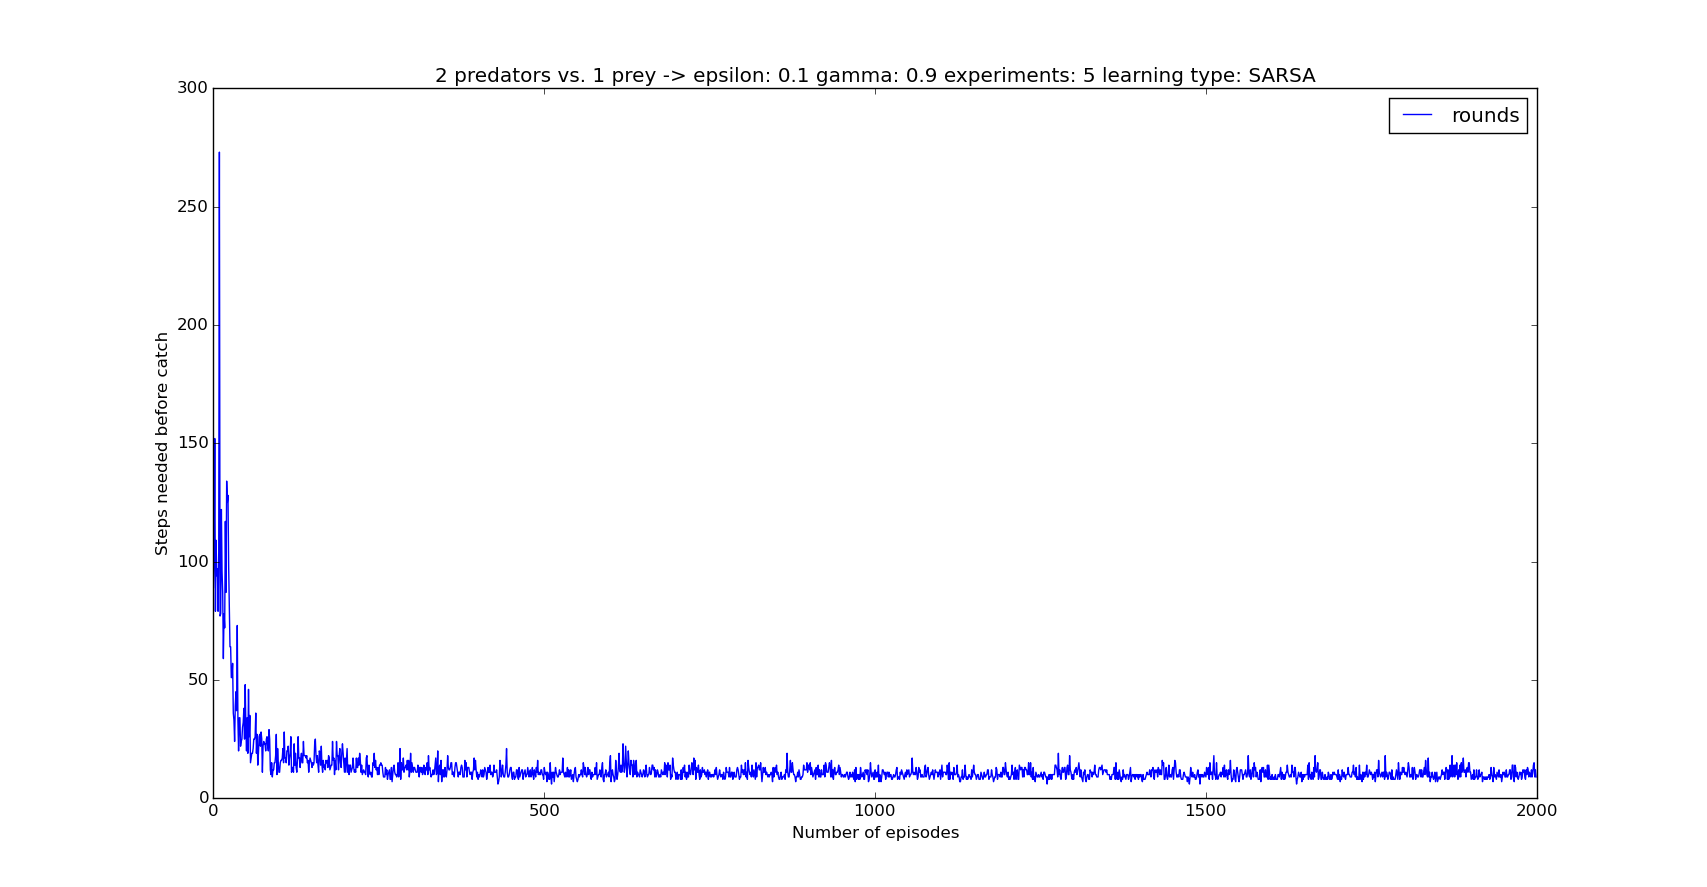
\includegraphics[scale=0.3]{1_predator_1_prey_SARSA}
	\captionof{figure}{Independent SARSA: 1 predator vs. 1 prey}
\end{center}

As seen with independent Q-learning, the predator learns how to catch the prey quicker than before. This confirms the theory that the smaller state space leads to quicker conversion of the algorithms. 

Compared to independent Q-learning, SARSA takes much longer to catch the prey in the beginning. Also, after learning the amount of rounds it takes the predators to catch the prey still vary much. However, where there is a spike rounds in Q-learning, there is not in SARSA. This happens due to the fact that SARSA is more careful than Q-learning. As SARSA is an on-policy learning algorithm, it is more careful than Q-learning. This leads to less extreme exploratory actions, choosing the "safe path" more often than Q-learning.

\subsubsection{2 predators vs. 1 prey}
\begin{center}
	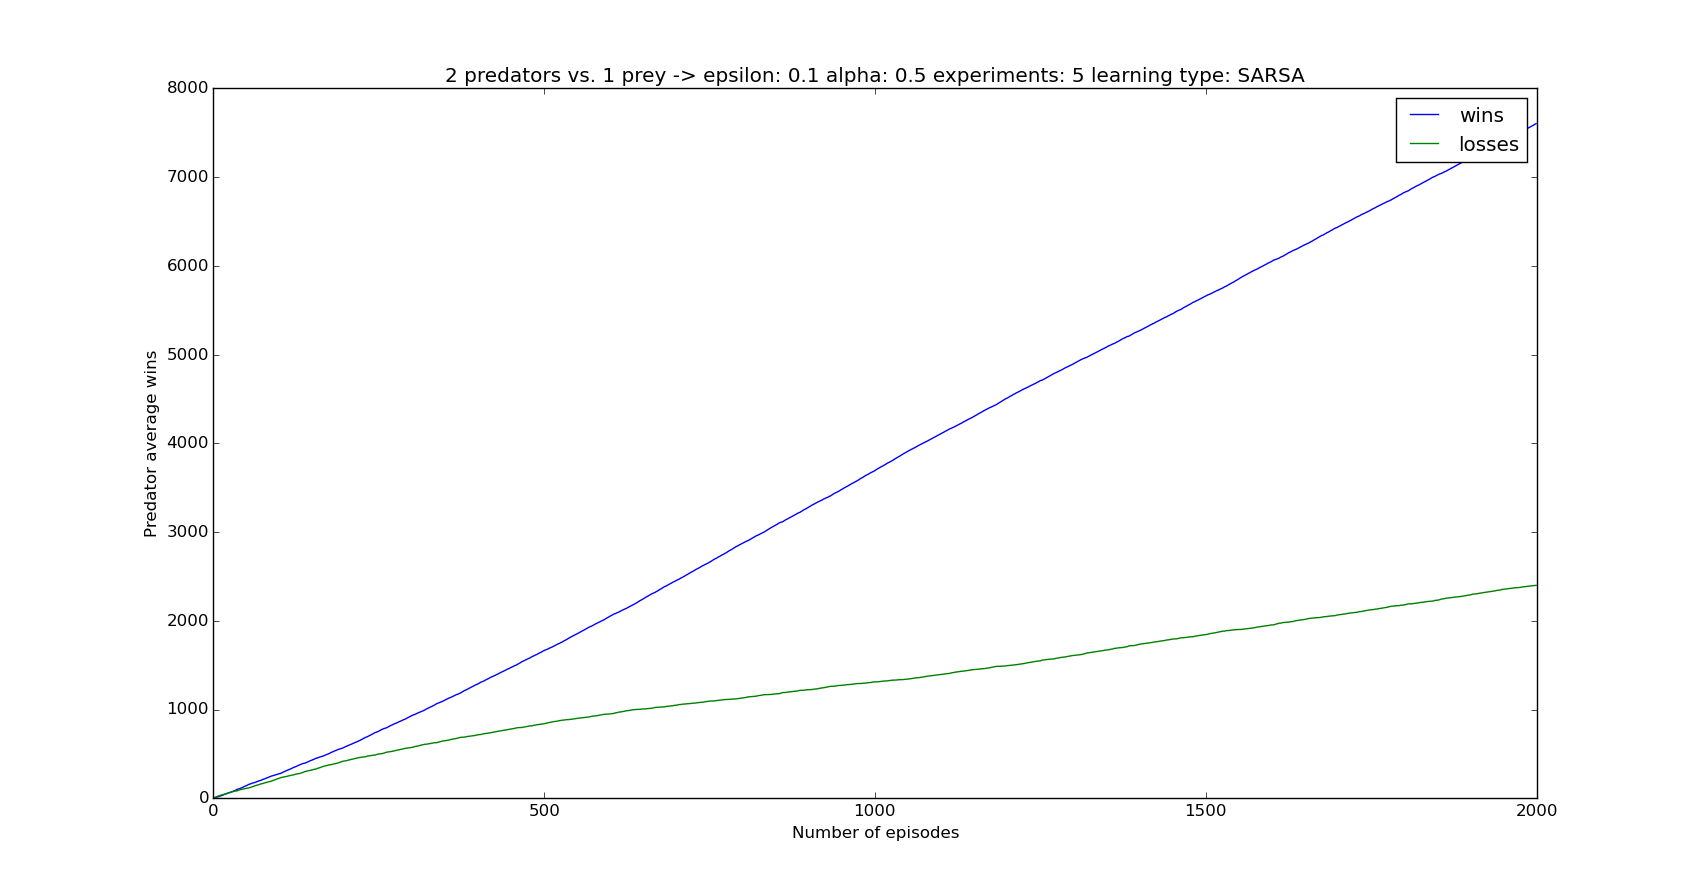
\includegraphics[scale=0.3]{2_predators_SARSA}
	\captionof{figure}{Independent SARSA: 2 predators vs. 1 prey}
\end{center}

The graph is very similar to the graph in Q-learning. This is possible, as both are temporal difference learning methods and are based on the same principles. The main difference between these two is that SARSA is an on-policy learning method and Q-learning is an off-policy learning method. It is therefore expected for these two methods to behave similarly.

\begin{table}[H]
\begin{center}
\begin{tabular}{| l | l | l | l | l |}
\hline
 & \parbox{2cm}{\textbf{Avg wins \\ (first 100)}} & \parbox{2cm}{\textbf{Avg losses \\ (first 100)}} & \parbox{2cm}{\textbf{Avg wins \\ (last 100)}} & \parbox{2cm}{\textbf{Avg losses \\ (last 100)}} \\
\hline
\textbf{Predators} & 55 & 44 & 78 & 21 \\
\hline
\end{tabular}
\caption{Average \# wins and losses by the predators}
\end{center}
\end{table}

Compared to independent Q-learning, independent SARSA performs slightly better. This can be attributed to the fact that SARSA is more careful than Q-learning. This behaviour leads to more wins for the predators.

\subsubsection{2 predators vs. 1 prey}
This is slooooow

\subsubsection{4 predators vs. 1 prey}
Again, this is intractable. 

\subsubsection{Parameter settings}
Again, parameter settings were explored for this algorithm.

\subsubsection{Learning rate}

\subsubsection{Discount factor}

\subsubsection{$\epsilon$-greedy action selection}